One of the core debates of economic theory is that of the rationality of agents. Keynesian economics was the dominant school of thought until the 1970s which saw the rise of New Classical economics\autocite{Hartley2013}. Lucas and Sargent were two key spearheads of this movement with their influential paper titled "After Keynesian Macroeconomics"\autocite{Lucas1979}, key to their complaints were the lack of microeconomic foundations in Keynesian models. Real business cycle theory, a major branch of New Classical economics believed that business cycles were a rational response to exogenous shocks to the economy and were perfectly efficient. However, this also meant that business cycles would not arise endogenously as firms and consumers would learn over time the behavior of the economy as they, as a whole, acted rationally. Though Keynesianism has since gained in popularity again, these lessons of New Classical Economics continue to influence the microfoundations of macroeconomic New Keynesian models.

Wegener, et al. directly based their inventory cycle model on that developed by Metzler. However, both of these models required that firms be boundedly rational which, to a New Classical economist, would be an unrealistic assumption not rooted in microeconomic foundations. However, it is appropriate to limit the ability for firms to predict the future if the reason for it can be appropriately explained. Behavioral economics and experimental data has frequently shown a gap between perfectly rational, utilitarian behavior and what is actually practiced by humans\autocite{Smith2006}; however, there is another mechanism that can be used to explain the inability for firms to behave rationally. Some models make use of stochastic shocks; these tend to follow a New Classical real business cycle framework as these stochastic processes are the primary drivers of economic cycles. Another possible process is that of chaotic behavior. Under these conditions, it is possible for the economy to reside in a completely deterministic state while still making it impossible for firms to accurately predict future states in the economy because in chaotic system, knowing the approximate current or past states does not mean that one knows the future state to any reasonable approximation. Having the unpredictability of the economy be primarily driven by chaotic processes rather than stochastic ones is of great use from a policy perspective, this is discussed in greater detail by Faggini and Parziale\autocite{Faggini2012}. 

The growth model described in Chapter \ref{ch:metzlerian-expanded} has a basis in Metzler's inventory cycle but also incorporates a multiplier-accelerator mechanism for endogenous investment and consumption and the results of numerical simulations of the model display the possibility of chaos, in addition to other phenomena such as the existence of multiple attractors. Of particular note is the bifurcation diagram and lyapunov exponent plot of the parameter $s$. The marginal propensity to save, under the initial conditions and other parameter choice tested, do not display any stable fixed points. In fact, over the possible range of $s$, most possible trajectories are chaotic; one such trajectory is displayed in Figure \ref{growth_chaotic-timeseries}.
\begin{figure}
    \centering
    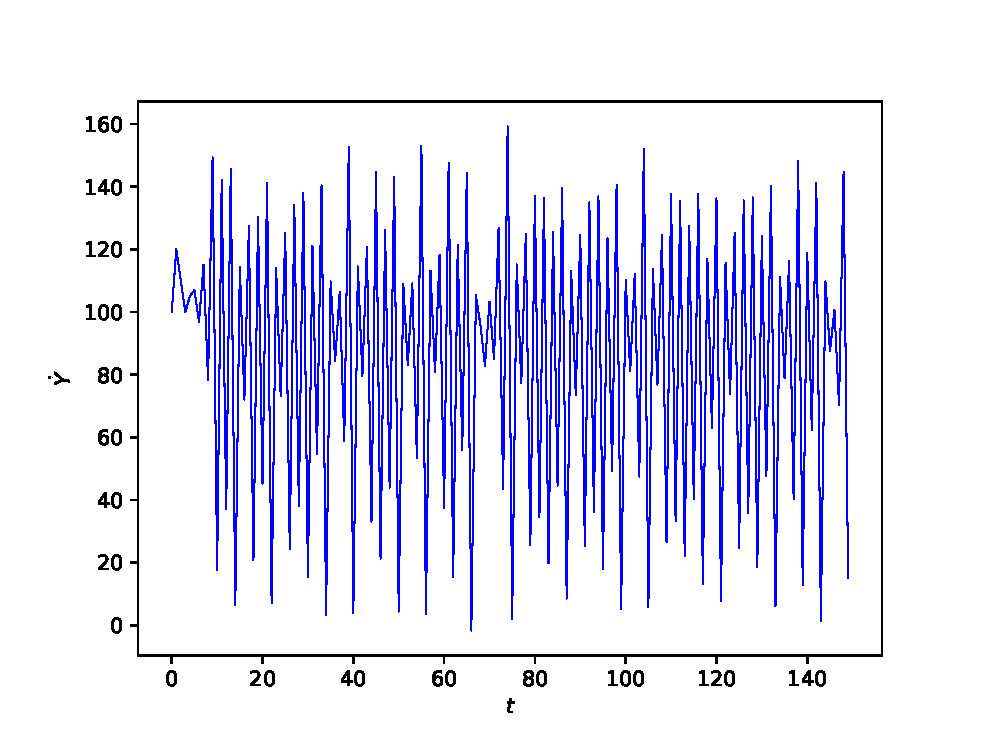
\includegraphics[height=0.4\textheight]{./metzlerian_growth/chaotic_timeseries.eps}
    \caption{Timeseries plot of income growth rate over 150 iterations. $s=0.4,\ k=0.3,\ v=500,\ q=0.001$. Initial values of $\dot Y$ are: 100, 120, 110, 100, 105, 107}
    \label{growth_chaotic-timeseries}
\end{figure}
Figure \ref{metzlerian_growth-klyapunov} also displays chaotic behavior; however, this only occurs when $k$ is very large and is unlikely to occur in a real scenario. Both $s$ and $k$ are the two parameter choices that describe the behavior of the agents of the economy in non-monetary terms. Based on the results of Figure \ref{metzlerian_growth-klyapunov} and \ref{metzlerian_growth-kbifurcation}, variation of this parameter has minor effects on the growth rate of the economy compared to variation of $s$. This implies that the choice of inventory proportion, outside of the extreme cases, has a minor impact on the long-run dynamics of the model. This is not to say that the inventory cycle is itself a minor factor of the economy; removal of the inventory cycle changes this model to an unsimplified version of the model presented in Chapter \ref{ch:multiplier-accelerator}. This model features a functionally identical mechanism for consumption with a Robertson lag and although the form of the function for endogenous investment differs between the two models, they are qualitatively similar for the reasons mentioned in Chapter \ref{ch:metzlerian-expanded}.

\begin{figure}
    \centering
    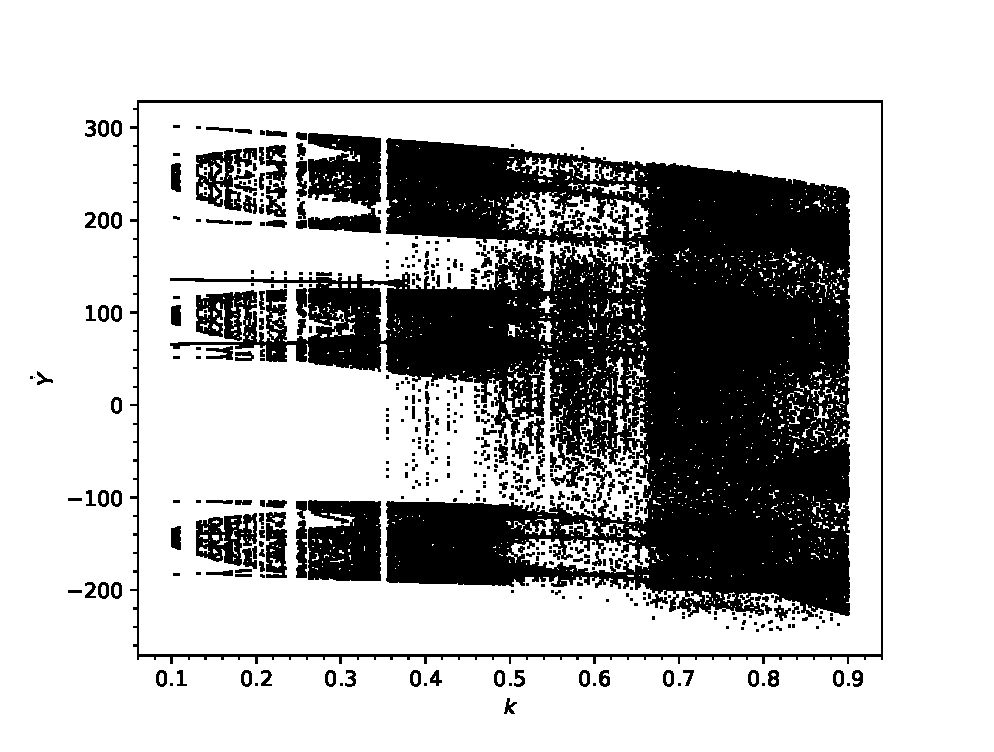
\includegraphics[height=0.4\textheight]{./metzlerian_growth/kbifurcation2.eps}
    \caption{Bifurcation diagram varying $k$ between 0.1 and 0.9. Initial conditions and other parameters are held constant as described in Figure 4.1 except $s=0.7$}
    \label{metzlerian_growth-kbifurcation2}
\end{figure}
\begin{figure}
    \centering
    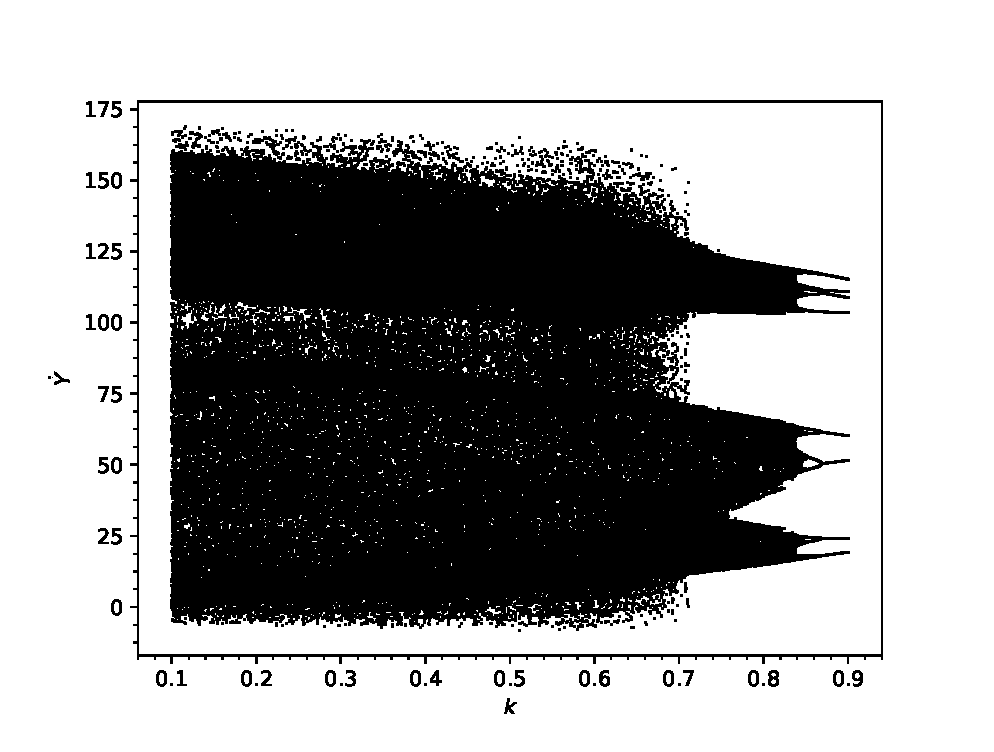
\includegraphics[height=0.4\textheight]{./metzlerian_growth/kbifurcation3.eps}
    \caption{Bifurcation diagram varying $k$ between 0.1 and 0.9. Initial conditions and other parameters are held constant as described in Figure 4.1 except $s=0.3$}
    \label{metzlerian_growth-kbifurcation3}
\end{figure}
Figure \ref{metzlerian_growth-kbifurcation2} and \ref{metzlerian_growth-kbifurcation3} displays behavior that is qualtiatively distinct from that in Figure \ref{metzlerian_growth-kbifurcation} despite both plots showing the long-run behavior of the model with the same variation in $k$. However, by increasing or decreasing $s$ until it is in the chaotic regime presented in Figure \ref{metzlerian_growth-slyapunov}, we see that varying $k$ can have a significant effect on the long-run dynamics of growth at even more reasonable values of $k$.

